\chapter{Entwicklungsumgebungs Perference Page}
\label{chap:settings}
Für die Entwicklungsumgebung wurde eine Eclipse Preference Page erstellt. In diesem Kapitel wird erklärt, welche Einstellungen in dieser Preference Page vorgenommen werden können und welche Auswirkungen diese haben. Die Einstellungen sind im Eclipse Preference Dialog unter MCore zu finden.
\section{Umbilical}

Der Umbilical-Port kann über einen Dialog, der alle möglichen Ports anzeigt, ausgewählt werden.

\begin{figure}[H]
	\centering
		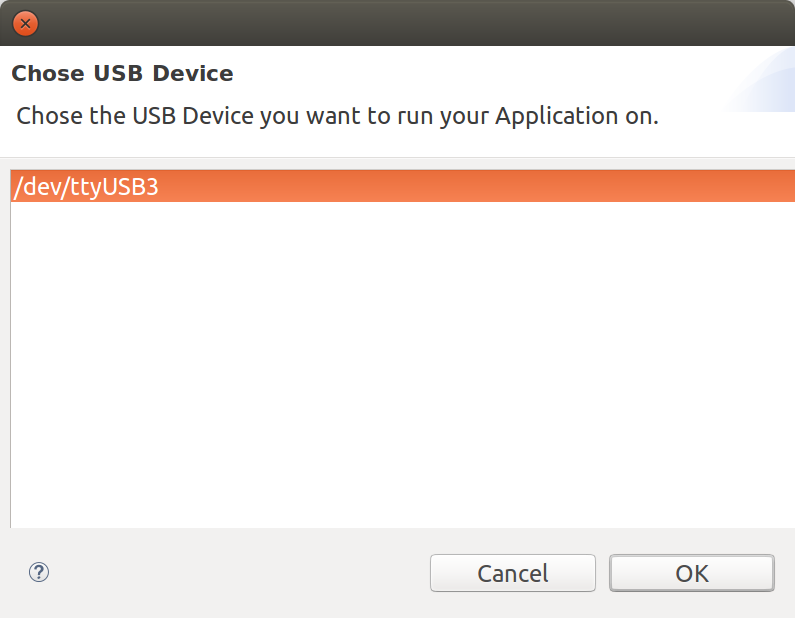
\includegraphics[scale=0.3]{idesettings/umbilical.png}
		\caption{Dialog, über welchen der Umbilical-Port gesetzt werden kann.}
		\captionsetup{margin=0cm,font={footnotesize}}
		\label{fig:umbilicalport}
\end{figure}

Der Port wird automatisch gesetzt, wenn das Programm ausgeführt wird. 

\section{Loader}

Der Loader ist das File, das von Forth mit dem Befehl
%
\begin{verbatim}
gforth ./loader.fs
\end{verbatim}
%
gestartet wird. Im Loader befindet sich ein Platzhalter \$INPUT\_FILE, der bei der Ausführung des Programms durch den Namen des Files ersetzt wird.